% Figura di testo: paper v4 Figure 1 (schema, nessun numero). TikZ.
\begin{figure}[tbp]
\centering
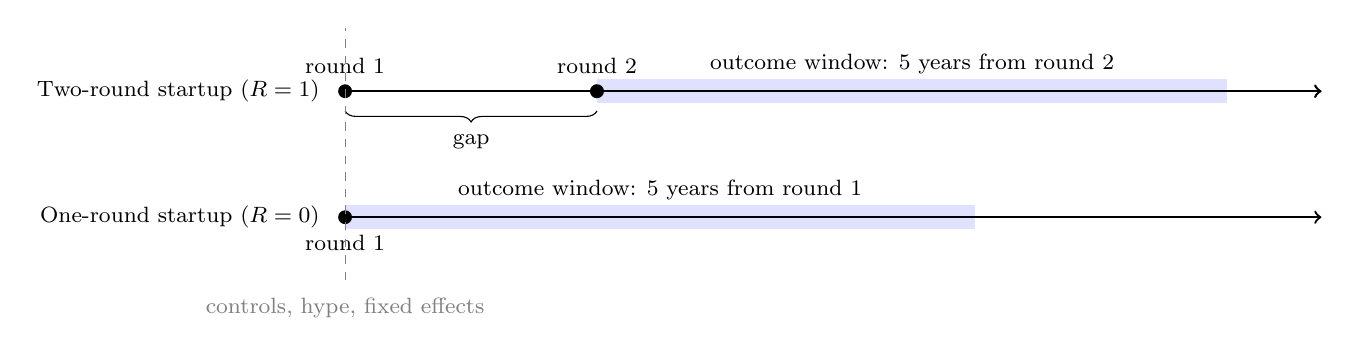
\begin{tikzpicture}[x=1cm,y=1cm,font=\footnotesize]
  % two-round startup
  \node[anchor=east] at (-0.2,1.6) {Two-round startup ($R=1$)};
  \draw[thick,->] (0,1.6) -- (12.4,1.6);
  \fill (0,1.6) circle (2.5pt) node[above=3pt] {round 1};
  \fill (3.2,1.6) circle (2.5pt) node[above=3pt] {round 2};
  \draw[decorate,decoration={brace,amplitude=4pt,mirror}] (0,1.35) -- (3.2,1.35) node[midway,below=5pt] {gap};
  \fill[blue!12] (3.2,1.45) rectangle (11.2,1.75);
  \draw[thick,->] (0,1.6) -- (12.4,1.6);
  \fill (3.2,1.6) circle (2.5pt);
  \node at (7.2,1.95) {outcome window: 5 years from round 2};
  % one-round startup
  \node[anchor=east] at (-0.2,0) {One-round startup ($R=0$)};
  \fill[blue!12] (0,-0.15) rectangle (8.0,0.15);
  \draw[thick,->] (0,0) -- (12.4,0);
  \fill (0,0) circle (2.5pt) node[below=3pt] {round 1};
  \node at (4.0,0.35) {outcome window: 5 years from round 1};
  % round-1 timing
  \draw[dashed,gray] (0,-0.8) -- (0,2.4);
  \node[gray,align=center] at (0,-1.15) {controls, hype, fixed effects};
\end{tikzpicture}
\caption{The two-group design and the timing of each variable}
\label{fig:F1}
\par\smallskip\parbox{0.95\linewidth}{\scriptsize Schematic, not to scale. For two-round startups the outcome window opens at round 2, so a startup enters the window only after surviving the gap; for one-round startups it opens at round 1. Controls, hype and fixed effects are dated at round 1.}
\end{figure}
